\documentclass[BTech]{nitkdiss}

\usepackage{amsmath,amssymb,graphicx,color,colortbl}
\usepackage{csquotes}
\begin{document}
\begin{center}
\section*{Certificate}
\end{center}
This is to certify that the project entitled \textbf{"Automatic Essay Evaluation"} submitted by : \\
\begin{center}
(1) Sai Chaitanya Banala (12EC25),\\
(2) Chetan Giridhar Vashisht (12EC31),\\
(3) Sharang Kulkarni (12EC85)
\end{center}
as the record of the work carried out by them, is \textit{accepted as the B. Tech Project Work Report Submission} in partial fulfilment of the requirements for the award of the degree of \textbf{Bachelor of Technology in Electronics and Communication Engineering}.\\ \\  
Guide
\\
\\
\\
Dr. Raghavendra Bobbi\\
Assistant Professor,\\
Department of Electronics and Communication Engineering.\\
National Institute of Technology Karnataka, Surathkal
\\
\\
\\
\\
Chairman-DUGC\\
(Signature with Date and Seal)







\title{Automatic Essay Evaluation}
\author{Sai Chaitanya Banala (12EC25)\\ Chetan Giridhar Vashisht (12EC31)\\ Sharang Kulkarni (12EC85)\\}
\mentor{Dr. Raghavendra Bobbi}
\date{\today}
\department{Electronics and Communication Engineering}




\maketitle

\singlespacing
\def\code#1{\texttt{#1}}
\newpage
\begin{abstract}
Standardized tests are hampered by the manual effort required to score student-written essays. Manual grading of students' essays is a time-consuming, labour-intensive and expensive activity for educational institutions. It is nevertheless necessary since essays are considered to be the most useful tool to assess learning outcomes. Automated essay evaluation represents a practical solution to this task. 

In this project we evaluate essays on a content based approach coupled with statistical substitutes using various algorithms. The data-set consisted of ≈13000 essays from Kaggle.com. These essays were divided into 8 different essay sets based on context. We combine simple, shallow features of the essays, such as character length and word length, with linguistic features. Our combined model gives significant reduction in prediction error. Quadratic weighting Kappa which measures agreement between predicted scores and human scores, was used as an error metric. Finally, we got insights into which features could improve the model. 

\end{abstract}

\newpage
\tableofcontents
\listoffigures
% \listoftables
\newpage
\pagestyle{plain}
\pagenumbering{arabic}

\chapter{Introduction}           
Essays are crucial testing tools for assessing academic achievement, integration of ideas and ability to recall but they are expensive and time consuming for states to grade them by hand.  So, we are frequently limited to multiple-choice standardized tests. We believe that automated scoring systems can yield fast, effective and affordable solutions that would allow states to introduce essays and other sophisticated testing tools.  We believe that you can help us pave the way towards a breakthrough.  

Analyzing natural language, or free-form text used in everyday human-to-human communications, is a vast and complex problem for computers regardless of the medium chosen, be it verbal communications,
writing, or reading. Ambiguities in language and the lack of one “correct” solution to any given communication task make grading, evaluating or scoring a challenging undertaking. In general, this is a perfect domain for the application of machine learning techniques with large feature spaces, and huge amounts of data containing interesting patterns.

This project
\begin{itemize}
    \item challenges us of automated student assessment systems to demonstrate their current capabilities.
    \item compare the efficacy and cost of automated scoring to that of human graders.
    \item reveal product capabilities and motivates people to adopt them.
\end{itemize}
\begin{figure}[h!]
\centering
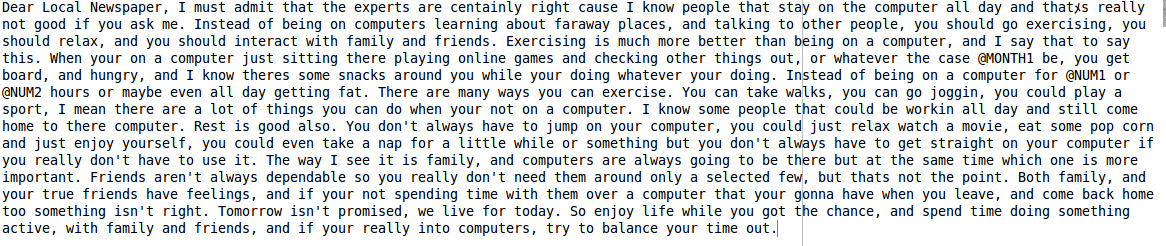
\includegraphics[scale=0.50]{snapshot2.png}
\caption{A typical essay}
\label{fig:Essay}
\end{figure}

\section{Motivation}
Our previous project on “Search Engine Relevance” using NLP techniques and statistical features motivated us into taking up a project in the same domain when we learnt that one of the key roadblocks to advancing school-based curricula focused on critical thinking and analytical skills is the expense associated with scoring tests to measure those abilities.  For example, tests that require essays and other constructed responses are useful tools, but they typically are hand scored, commanding considerable time and expense from public agencies.  So, because of those costs, standardized examinations have increasingly been limited to using “bubble tests” that deny us opportunities to challenge our students with more sophisticated measures of ability.

\chapter{Previous Work}
During our previous semester we went with the relevance of results yielded by search engines. This was a completed competition on Kaggle and the solutions were available to the public. The purpose of the project was to get us acquainted with basic NLP tools and ensemble modelling.\\

Based on the product title and the description of the product given by the search engine, we are supposed to rate how relevant it is to the query on a scale of 1 to 4. 4 being the most relevant. The metric of measurement used here was the quadratic weighing kappa. This metric penalises the square of the difference from the original result.\\

\section{Preprocessing}
\subsection{HTML tag dropping}
HTML tags are dropped to make it convenient for further processing.
		
\subsection{Synonym replacement and spelling correction}
These include changing certain words in the text to maintain uniformaty within the whole text. For example, children's, childerns', childrens, children, child', child, child's and kid are all replaced by kid.

\subsection{Stemming}
Stemming refers to changing words to their root forms i.e removal of extensions like -ly, -ing, -ed etc. Stemming is performed using nltk's built in package \code{nltk.stem.PorterStemmer()}.

\subsection{Enumeration of Query IDs}
Each of the query entries from the dataset are mapped to a query id in a 261 range of numbers.

\section{Feature Extraction}
Feature Extraction is performed on the entire dataset, to get some numbers out of the text inputs. The basic feature extraction can be divided into four parts, Counting features, Distance features, TF-IDF features and other miscellaneous features. The first step is extraction of n-grams $(n = {1, 2, 3})$ i.e unigrams, bigrams and trigrams from each data sample.\\
Example : {A blue LED strip}\\
\textbf{Unigrams}: \{A, blue, LED, strip\}\\
\textbf{Bigrams}: \{A blue, blue LED, LED strip\}\\
\textbf{Trigrams}: \{A blue LED, blue LED strip\}\\
The tuple $(q_i, t_i, d_i)$ denotes the $i^{th}$ sample of \code{query}, \code{product\_title} and \code{product\_description} respectively. $r_i$ and $v_i$ are the \code{median\_relevence} (training labels) and \code{relevence\_variance} respectively.

\subsection{Counting Features}
We plan to generate several counting features related the tuple $(q_i, t_i, d_i)$ of the $i^{\textrm{th}}$ data sample. $a_i$ refers to any of the components of the tuple $(q_i, t_i, d_i)$.

\subsection{Basic Counting Features}
\begin{itemize}
\itemsep -1em 
\item \textbf{Count of $n$-grams} i.e ngram$(a_i, n)$.\\
\item \textbf{Count and Ratio of Digits in $a_i$.}\\
\item \textbf{Count and Ratio of Unique $n$-grams in $a_i$.}\\
\item \textbf{Binary indicator indicating whether description field $d_i$ is empty.}
\end{itemize}

\subsection{Intersect Counting Features}
\textbf{Count and Ratio of $a'$s $n$-gram in $b'$s $n$-gram}
such features are computed for all the combinations of $a \in {\{q_i, t_i, d_i\}}$ and $b \in{\{q_i, t_i, d_i\}}$, $(a\neq b)$.

\subsection{Intersect Position Features}
\textbf{Statistics of Positions of $a$'s $n$-gram in $b$'s $n$-gram}\\ For those intersect $n$-gram, their positions are computed and the following statistics are taken as features.\\
\begin{itemize}
\itemsep 0 em 
\item \textbf{Minimum value} (0\% quantile)
\item \textbf{Median value} (50\% quantile)
\item \textbf{Maximum value} (100\% quantile)
\item \textbf{Mean value}
\item \textbf{Standard deviation}
\item \textbf{Statistics of Normalized Positions of $a$'s $n$-gram in $b$'s $n$-gram}
\end{itemize}

\subsection{Distance Features}
Defining two new distance metrics, for two \code{sets} $A$ and $B$,
$$\textrm{JaccardCoef}(A, B) = \frac{|A\cap B|}{|A \cup B|}$$
and
$$\textrm{DiceCoeff}(A,B) = \frac{2|A \cap B|}{|A| + |B|}$$
These are new metrics which are used later for the purpose of distance calculations. 
\subsection{Basic Distance Features}
The following distances are computed as features\\
\textbf{D(ngram$(q_i, n)$, ngram$(t_i, n)$)}\\
\textbf{D(ngram$(q_i, n)$, ngram$(d_i, n)$)}\\
\textbf{D(ngram$(t_i, n)$, ngram$(d_i, n)$)}\\
where D$(. , .)\in\{\textrm{JaccardCoef}(\textrm{set}(.), \textrm{set}(.)), \textrm{DiceDist}(\textrm{set}(.), \textrm{set}(.))\}$, and $\textrm{set}(.)$ converts
the input \code{list} to a \code{set}.

\subsection{TF-IDF features}
This is the most important set of features. The result of TFIDF features is an ultra sparse matrix on which we operate later. There are two sets of TFIDF features extracted from the dataset. In the first case we concatenate the \code{query} with the \code{product\_title} and extract the features from this one. For the second case, we concatenate the \code{query}, the {product\_title} and the \code{product\_description}. We then feed each of the extracted features to two separate pipelines.

\section{Pipeline Architecture and Model Building}
\begin{figure}[h!]
\centering
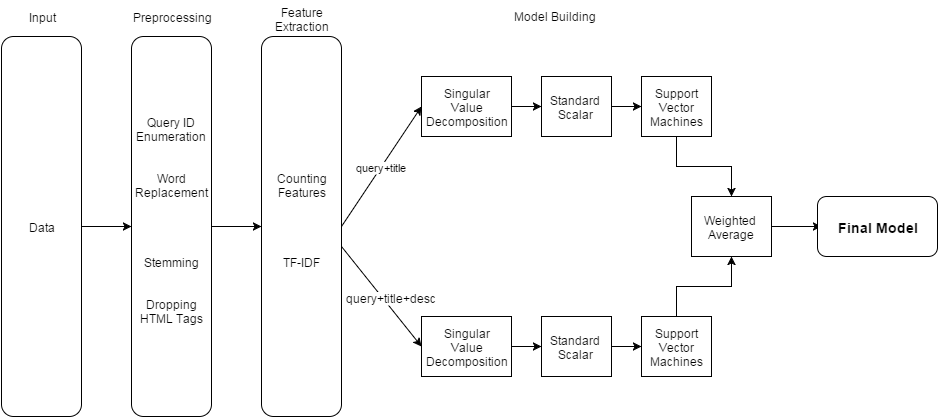
\includegraphics[scale=0.50]{flowchart.png}
\caption{Flow of the project}
\label{fig:flowchart}
\end{figure}
The extracted features are fed to a pipeline where we conduct a \code{grid search} to find the optimal set of parameters for the cost function(The \code{quadratic weighing kappa}). The stages for the pipeline are as follows.
\begin{itemize}
\item{Singular Value Decomposition}
\item{Standard Scalar}
\item{Support Vector Machine}
\end{itemize}
\section{Singular Value Decomposition(SVD)}
We use \code{SVD} to reduce the dimensionality of our feature space from an ultra sparse matrix to 300 components.
\subsection{Standard Scalar (SS)}
Normalisation is conducted on the new feature space, via \code{mean normalisation}. This ensures that all components are within the same range, so that operations conducted on them later (like \code{Euclidean distance}) will not give an dimension any extra weight age.
\subsection{Support Vector Machine(SVM)}
The last stage of the pipeline is an SVM where the new feature set is fed. The classifier attempts to classify based on the cost function.
\subsection{Grid Search}
We fit the pipeline onto the dataset and then conduct a parameter wide grid search to determine the most feasible set of parameters to optimise our cost function. Upon conducting a grid search on both the pipelines we get two fitting models. 
\subsection{Ensemble Average}
We get two SVM models, one from each pipeline. The accuracies of both models are 0.54 and 0.56 respectively. The ensemble average of two yields 0.63. The ensemble average used here is the arithmetic mean.
\section{Conclusions}
On using an ensemble model we obtain a relevance score of 0.63 in under ten minutes of computation. Although this not as good as the one done by the winners (0.71), it takes mush lesser time to compute the output. The time requirements are over five hours for the winning solution. Here is a sample confusion matrix genrated after the ensemble model.\\\\
$C = 
\begin{pmatrix}
150 & 35 & 2 & 1\\
65 & 200 & 65 & 11\\
2 & 47 & 185 & 92\\
9 & 51 & 354 & 1200\\
\end{pmatrix}$
%---------------------------------------------------%

\chapter{Literature Survey}
\section{Our Approach}
We are implementing a paper and adding some of our own ideas to the rating system. The main paper that we are referring to is \textit{Modeling Argument Strength in Student Essays}.\\

A major weakness of many existing scoring engines such as the Intelligent Essay Assessor is that they adopt a holistic scoring scheme, which summarizes the quality of an essay with a single score and thus provides very limited feedback to the writer. In particular, it is not clear which dimension of an essay (e.g., style, coherence, relevance) a score should be attributed to. Recent work addresses this problem by scoring a particular dimension of essay quality such as coherence, technical errors, relevance to prompt (Higgins et al., 2004; Persing and Ng, 2014), organization (Persing et al., 2010), and thesis clarity. Essay grading  software that provides feedback along multiple dimensions of essay quality such as E-rater/Criterion has also begun to emerge.\\

We aim to develop a computational model for scoring the essay dimension of argument strength, which is arguably the most important aspect of argumentative essays. Argument strength refers to the strength of the argument an essay makes for its thesis. An essay with a high argument strength score presents a strong argument for its thesis and would convince most readers. While there has been work on designing argument schemes for annotating arguments manually and automatically in student essays, little work has been done on scoring the argument strength of student essays. It is worth mentioning that some work has investigated the use of automatically determined argument labels for heuristic and learning-based essay scoring, but their focus is holistic essay scoring, not argument strength essay scoring.


\section{Concepts and methods}
Automatic essay evaluation mainly revolves around three models of feature extraction and classification.\\

Automated scoring of textual response thus requires as its fundamental prerequisite a complex of techniques which address the full linguistic structure of texts (and thus the full verbal capacity of test subjects) to a greater or lesser extent, and with greater or lesser inferential complexity. Approaches to the scoring of textual responses to be discussed in this chapter involve three types of 2 linguistic analyses:\\

\textit{Linguistic feature-based methods} In these approaches, specific linguistic features are extracted from target texts and regression analyses are performed to determine their correlation with variables that summarize performance in a task that is conceptually meaningful or that correlates with measures of student proficiency as gauged by a criterion such as human raters or performance on other tasks. In this class of methods, the focus is on both extracting features and summarizing them at the level of individual task performances. The features that are being extracted correspond to construct-level categories, that is, to categories of linguistic structure, such as particular grammatical constructions, particular classes of words, or other construct-level generalizations over language structure.\\

\textit{Vector space methods} These include Latent Semantic Analysis. These approaches construct a vector model over large quantities of linguistic information and use cosine distance (or some other metric on the vector space) as the basis of an empirically derived predictive model. In this class of methods, the focus is on a mathematical summary of features, where features may be as simple as the vector of counts of words used. Such methods can be distinguished from feature-based methods in that they employ no direct representation of construct-level categories. Generalizations about construct structure emerge from the mathematical summary of the features and not from the features themselves.

\textit{Linguistic structure analysis} In these approaches, natural language processing techniques are applied to build a (partial) model of the mental representations associated with task-relevant constructs, and these representations are used in turn to predict task-relevant constructs. The natural language processing techniques can vary from relatively simple information extraction techniques, where the focus is on identifying recurrent patterns, to full sentence and discourse parsing with semantic interpretation. What distinguishes linguistic analysis of this sort from simpler methods is that the analysis extracts a structure, a set of elements and their relations, rather than simple quantifiable properties such as word counts or the frequency of
construct categories.\\

Project Essay Grade uses a linguistic based model to extract features. The Intelligent Essay Assessor primarily uses Latent Semantic Analysis and E-rater uses a combination of feature analysis, vector space models and linguistic analysis.

\section{Results on Kaggle}
The competition on Kaggle was completed in April 2012. The results announced here are compared by Ben Hamner. He compares the various approaches used by the winning teams and their accuracies. All the solutions of the winners are a secret and have not been published. They were awarded by the Hewlett Foundation. Quoting from \textit{Contrasting State-of-the-Art Automated Scoring of Essays Analysis}

\begin{displayquote}
Six of the eight essays were transcribed from their original handwritten responses using two transcription vendors. Transcription accuracy rates were computed at 98.70\% for 17,502 essays.  The remaining essays were typed in by students during the actual assessment and provided in ASCII form. Seven of the eight essays were holistically scored and one employed score assignments for two traits. Scale ranges, rubrics, and scoring adjudications for the essay sets were quite variable. Results were presented on distributional properties of the data (mean and standard deviation) along with traditional measures used in automated essay scoring: exact agreement, exact+adjacent agreement, kappa, quadratic weighted kappa, and the Pearson $r$. The results demonstrated that overall, automated essay scoring was capable of producing scores similar to human scores for extended-response writing items with equal performance for both source-based and traditional writing genre. Because this study incorporated already existing data (and the limitations associated with them), it is highly likely that the estimates provided represent a floor for what automated essay scoring can do und
er operational conditions.
\end{displayquote}

There are several arguments against the use of machine learning for automatic essay evaluation, especially in this competition. Quoting from Critique (Ver. 3.4) of Mark D. Shermis \& Ben Hamner, “Contrasting State of the Art Automated Scoring of Essays: Analysis”

\begin{displayquote}
Although the unpublished study by Shermis \& Hammer (2012) received substantial publicity about its claim that automated essay scoring (AES) of student essays was as accurate as scoring by human readers, a close examination of the paper’s methodology and the data sets used demonstrates that such a claim is not supported by the data in the study. The study’s methodology used one variable for comparing human readers and a different variable for comparing machine scores, this difference artificially privileging the machines in half the datasets. Moreover, conclusions were drawn without the performance of statistical tests and inferences were based solely on impressionistic and sometimes inaccurate comparisons. In addition, there was no standard testing of the model as a whole for significance, which given the large number of comparisons, allowed machine variables to surpass human readers merely through random chance. Finally, half of the datasets used were not essays but short one paragraph responses involving literary analysis or reading comprehension that were not evaluated on any construct involving writing.  Because of the widespread publicity surrounding this study and that its findings may be used by states and state consortia in implementing the Common Core State Standards Initiative, the authors should make the test dataset publicly available for analysis.
\end{displayquote}


\chapter{Data and Evaluation}
For this project,we used the data-sets from a competition hosted on Kaggle. There are eight essay sets. Each of the sets of essays was generated from a single prompt. Selected essays range from an average length of 150 to 550 words per response. Some of the essays are dependent upon source information and others are not. All responses were written by students ranging in grade levels from Grade 7 to Grade 10. All essays were hand graded and were double-scored. Each of the eight data sets has its own unique characteristics. 

\section{Dataset}
The dataset contains the following columns\\
\code{essay\_id} : A unique identifier for each individual student essay.\\
\code{essay\_set} : 1-7, an id for each set of essays.\\
\code{essay} : The ascii text of a student's response.\\
\code{rater 1} : Rater 1's score.\\
\code{rater 2} : Rater 2's score.\\

\section{Anonymization}

All the personally identifying information was removed from the essays using the Named Entity Recognizer (NER) from the Stanford Natural Language Processing group and a variety of other approaches. The relevant entities are identified in the text and then replaced with a string such as "@PERSON1."

The entitities identified by NER are: "PERSON", "ORGANIZATION", "LOCATION", "DATE", "TIME", "MONEY", "PERCENT"

Other replacements made: "MONTH" (any month name not tagged as a date by the NER), "EMAIL" (anything that looks like an e-mail address), "NUM" (word containing digits or non-alphanumeric symbols), and "CAPS" (any capitalized word that doesn't begin a sentence, except in essays where more than 20\% of the characters are capitalized letters), "DR" (any word following "Dr." with or without the period, with any capitalization, that doesn't fall into any of the above), "CITY" and "STATE" (various cities and states).

Here are some hypothetical examples of replacements made:
\begin{itemize}
\item{"I attend Springfield School..." $-->$ "...I attend \@ORGANIZATION1"}
\item{"once my family took my on a trip to Springfield." $-->$ "once my family took me on a trip to \@LOCATION1"}
\item{"John Doe is a person, and so is Jane Doe. But if I talk about Mr. Doe, I can't tell that's the same person." $-->$ "...\@PERSON1 is a person, and so is PERSON2. But if you talk about \@PERSON3, I can't tell that's the same person."}
\item{"...my phone number is 555-2106" $-->$ "...my phone number is \@NUM1"}
\end{itemize}
Any words appearing in the prompt or source material for the corresponding essay set were white-listed and not anonymized.



\section{Evaluation}
Essay score predictions are evaluated using objective criteria.

Specifically, the performance is evaluated with the quadratic weighted kappa error metric, which measures the agreement between two raters.  This metric typically varies from 0 (only random agreement between raters) to 1 (complete agreement between raters).  In the event that there is less agreement between the raters than expected by chance, this metric may go below 0.  The quadratic weighted kappa is calculated between the automated scores for the essays and the resolved score for human raters on each set of essays.  The mean of the quadratic weighted kappa is then taken across all sets of essays.  This mean is calculated after applying the Fisher Transformation to the kappa values.

A set of essay responses E has N possible ratings, $1, 2,.., N$ and two raters, Rater $A$ and Rater $B$.  Each essay response $e$ is characterized by a tuple $(e_a,e_b)$, which corresponds to its scores by Rater $A$ (resolved human score) and Rater $B$ (automated score).  The quadratic weighted kappa is calculated as follows.  First, and $N$-by-$N$ histogram matrix $O$ is constructed over the essay ratings, such that $O_{i,j}$ corresponds to the number of essays that received a rating $i$ by Rater $A$ and a rating $j$ by Rater $B$.

An $N$-by-$N$ matrix of weights, $w$, is calculated based on the difference between raters’ scores:
$$w_{i,j} = \frac{(i-j)^2}{(N-1)^2}$$
An $N$-by-$N$ histogram matrix of expected ratings, $E$, is calculated, assuming that there is no correlation between rating scores.  This is calculated as the outer product between each rater’s histogram vector of ratings, normalized such that $E$ and $O$ have the same sum.

From these three matrices, the quadratic weighted kappa is calculated: 
$$\kappa = 1 - \frac{\sum_{i,j}^{}w_{i,j}O_{i,j}}{\sum_{i,j}^{}w_{i,j}E_{i,j}}$$

The Fisher Transformation is approximately a variance-stabilizing transformation and is defined:

$$z=\frac{1}{2}\ln{\frac{1+\kappa}{1 - \kappa}}$$

Since this transformation approaches infinity as kappa approaches 1, the maximum kappa value is capped at 0.999.  Next the mean of the transformed kappa values is calculated in the z-space.  For Essay Set 2, which has scores in two different domains, each transformed kappa is weighted by 0.5.  This means that each dataset has an equally weighted contribution to the final score.  Finally, the reverse transformation is applied to get the average kappa value:

$$ \kappa=\frac{e^{2z}-1}{e^{2z}+1}$$

\chapter{Feature Extraction}
Since the essays are all rated on a different scale, the training file is first split into eight different files (split according to the essay set). Then, the features are extracted on each of the files and stored to use in the future. Instead of extracting the same features repeatedly, we append the new features extracted to the existing file. (extracting the features is costly as it takes 1.5 seconds per essay and there are over ten thousand essays)

The evaluation metric for the project is the quadratic weighing kappa. This metric penalises the square of the difference between the scores of the rater and the prediction. 

Statistical features, grammatical features, argument based features and miscellaneous features are the broad types of features extracted.

\section{Statistical features}
These statistical substitutes are used to judge how well the students write their essays. This works as there is a very strong correlation between a person with good english and person who writes good essays
\begin{itemize}
    \item Number of sentences
	\item Number of words
	\item Number of unique words
	\item Number of long words
	\item Number of punctuations used (commas, brackets, quotes)
\end{itemize}


\section{Grammatical features}
The wealth of the grammar used by the author is explored using grammatical features. These give a good idea about proficiency of the user. Generally a person with good grammar writes good essays.

\begin{itemize}
    \item Number of spelling errors (using enchant)
	\item Parts of speech tagging, number of nouns, verbs, adverbs and adjectives
\end{itemize}
\newpage

\section{Linguistic model}
Apart from the statistical features of the text of each essay (such as the total number of words), linguistic features enable us to evaluate essays based on their argument strength. Various features of the essay, such as the Semantic Frames, Transitional Phrases, co-reference, adherence to the prompts topic, take model closer to duplicating human insight while grading essays.

\subsection{Transitional phrases}
14 transitional categories identified and the ngrams of the words are classified into these categories. The total count of each category is taken into account. The categories are:
    \begin{itemize}
        \item Addition: also, again, besides, similarly
		\item Consequence: accordingly, as a result
		\item Contrast: accordingly, otherwise
		\item Direction: here, there
		\item Diversion: by the way, incidentally
		\item Emphasis: above all, chiefly
		\item Exception: other than, outside of
		\item Exemplifying: chiefly, for instance
		\item Generalizing: as a rule, as usual
		\item Illustration: for example, for instance
		\item Similarity: comparatively, coupled with
		\item Restatement: in essence, in other words
		\item Sequence: at first, secondly
		\item Summarizing: after all, alas
    \end{itemize}
There are 149 phrases that have been accounted and placed into the above categories. 
\subsection{Content based}
Finding points in the essay which the raters would otherwise. To do this we construct a set of points (n grams) that acts as a dictionary. An exhaustive list of phrases is then compiled by finding synonyms of the existing dictionary. 

We look through each essay, once the content dictionary is built and look for matching phrases. A count of the matching phrases is collected as a feature.

\subsection{Co-reference features}
A strong argument must be cohesive so that the reader can understand what is being argued. While the transitional phrases already capture one aspect of this, they cannot capture when transitions are made via repeated mentions of the same entities in different sentences. We therefore introduce a set of co-reference features that capture information such as a fraction of essay's sentences that mention entities introduced in the prompt and the average number of total mentions per sentence.

\subsection{Semantic frames}
For each essay in our data set, we identify each semantic frame occurring in the essay as well as each frame element that participates in it. For example, a semantic frame may describe an event that occurs in a sentence, and the vent’s frame elements may be the people or objects that participate in the event. For example, given a sentence like "Mary sold the book to John", the task would be to recognize the verb "to sell" as representing the predicate, "Mary" as representing the seller (agent), "the book" as representing the goods (theme), and "John" as representing the recipient. This is an important step towards making sense of the meaning of a sentence. A semantic representation of this sort is at a higher-level of abstraction than a syntax tree. For instance, the sentence "The book was sold by Mary to John" has a different syntactic form, but the same semantic roles.

\subsection{Prompt Argument}:
Measure the strength of the argument from the introduction and conclusion of the paragraph mentioned. This feature is not useful for all the essay sets.
\begin{figure}[h!]
\centering
\includegraphics[scale=0.45]{extracted_features.png}
\caption{List of the some of the features extracted}
\label{fig:Essay}
\end{figure}

\chapter{Classification}
After all the features are stored into different files, we run two machine learning algorithms on the data to obtain different levels of accuracy for each of the essay sets. A parameter sweep is conducted across the entire dataset to obtain the best set of classifiers to use.

\begin{figure}[h!]
\centering
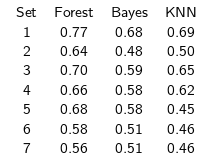
\includegraphics[scale=0.90]{snapshot1.png}
\caption{Results during mid evaluation}
\label{fig:Median relaveance}
\end{figure}

We choose the default parameters for both the Bayes learning algorithm and the Forest classifier. The forest classifier gives better results for the features extracted. 

\begin{figure}[h!]
\centering
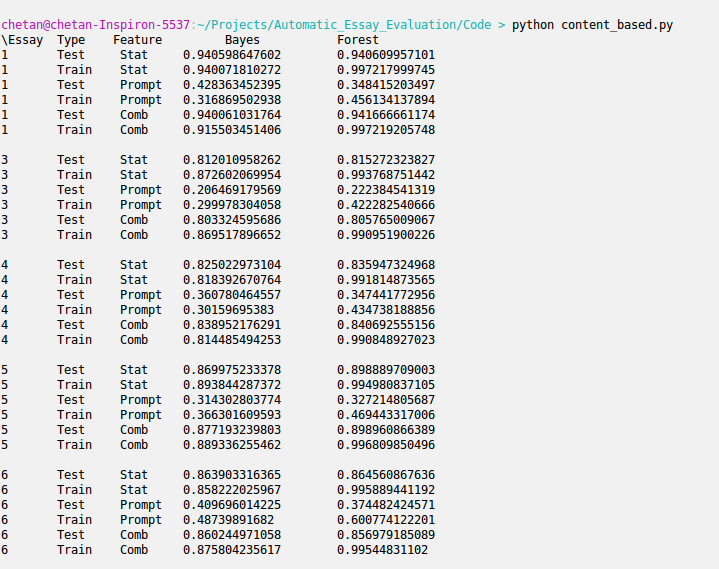
\includegraphics[scale=0.90]{output.png}
\caption{The new results over each essay set}
\label{fig:results}
\end{figure}

\chapter{Conclusions}
We proposed a feature-rich approach to the new problem of predicting argument strength scores on student essays. After, we implement a linguistic based approach and a statistical based approach to compare both the systems.\\

We have currently extracted over 40 features (a mixture of statistical, grammatical and linguistic)and the results with extracted features are documented above. The forest classifier gives the best results among the different machine learning algorithms used. The classifier gives over 80\% accuracy for each of the five essay sets. \\

\begin{figure}[h!]
\centering
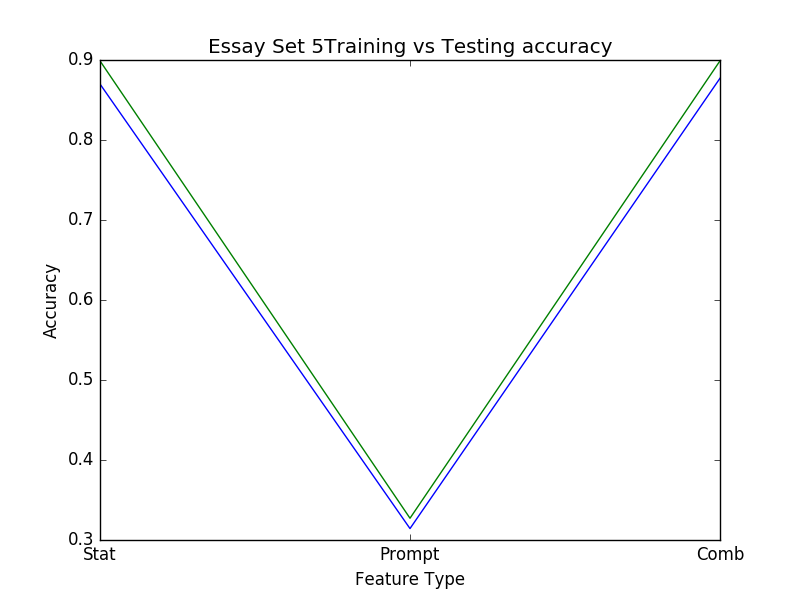
\includegraphics[scale=0.70]{5TrainVTest.png}
\caption{The testing accuracies for fifth essay set on the different feature spaces}
\label{fig:set5}
\end{figure}

The purpose of the project was to explore the gains in using the content-linguistic model. It takes very little time to grade the essays using a linguistic approach, once the model has been set up (10ms). The speed however comes at the cost of accuracy. The accuracy of the content models is no more than 40\% while statistical models give over 80\% consistantly. Adding this to the other model does not raise the accuracy considerably.

\begin{figure}[h!]
\centering
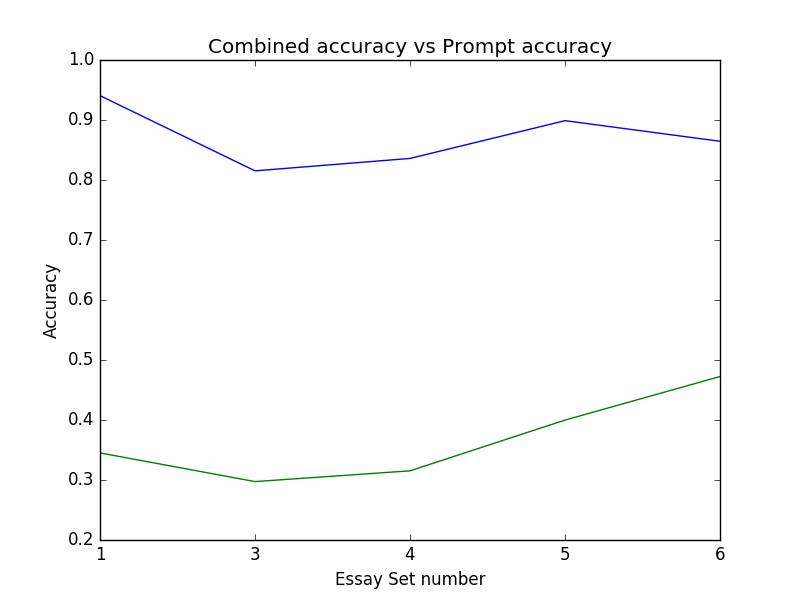
\includegraphics[scale=0.70]{CombVPrompt.png}
\caption{Testing accuracies for The Combination model vs the Prompt model}
\label{fig:CombVPrompt}
\end{figure}

We can see that the training accauracies are consistantly over 95\% and the testing accuracy is over 80\%. 

\begin{figure}[h!]
\centering
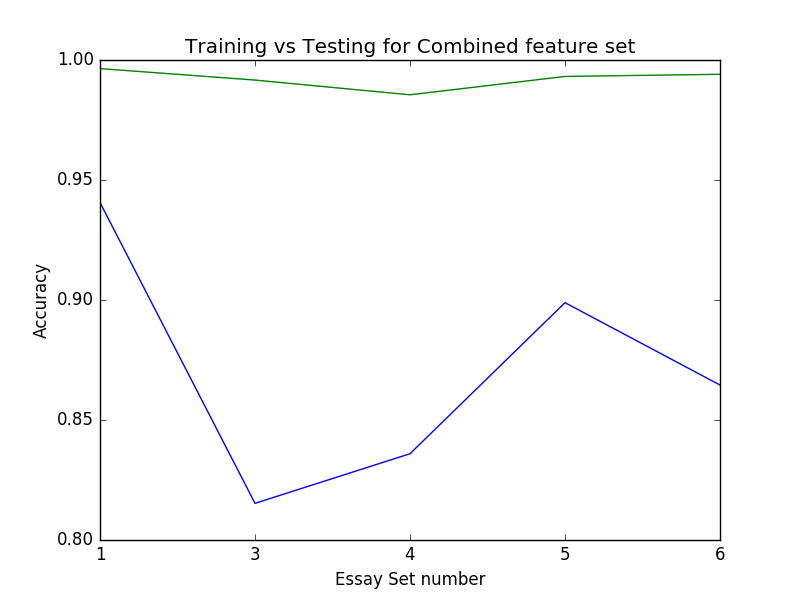
\includegraphics[scale=0.70]{TrainVTestComb.png}
\caption{Training vs Testing accuracy for the combined feature set}
\label{fig:CombVPrompt}
\end{figure}

\begin{thebibliography}{9}
\bibitem{Isaac Persing and Vincent Ng} 
Isaac Persing and Vincent Ng
\\\texttt{Modeling Argument Strength in Student Essays}

\bibitem{Manvi Mahana} 
Manvi Maha, Mishel Johns, Ashwin Apte
\\\textit{Automatic Essay Grading Using Machine Learning}

\bibitem{Andrew Kachites McCallum.}
2002. MALLET: A Machine Learning for Language Toolkit.
\\\textit{http://mallet.cs.umass.edu.}

\bibitem{Transitional Phrases}
Transitional Phrases, study guides and Strategies
\\\textit{http://www.studygs.net/wrtstr6.htm}

\bibitem{Derrick Higgins}
Derrick Higgins, Jill Burstein, Daniel Marcu, and Claudia Gentile.
\\\textit{2004. Evaluating multiple aspects of coherence in student essays}

\bibitem{Das Et Al}
Dipanjan Das, Nathan Schneider, Desai Chen, and Noah A. Smith. 2010.
\\\textit{Probabilistic frame-semantic parsing.}

\bibitem{SEMAFOR}
Dipanjan Das, Sam Thomson, Meghana Kshirsagar, André F. T. Martins, Nathan Schneider, Desai Chen, and Noah Smith. 
\\\textit{Semafor, a frame semantic parser, http://www.cs.cmu.edu/~ark/SEMAFOR/}

\bibitem{Contrasting State-of-the-Art Automated Scoring of Essays: Analysis}
Mark D. Shermis, Ben Hamner
\\\textit{Contrasting State-of-the-Art Automated Scoring of Essays: Analysis}

\bibitem{Critique}
Les C. Perelman, Ph.D.
\\\textit{Critique of Mark D. Shermis \& Ben Hammer, “Contrasting State of the Art Automated Scoring of Essays: Analysis"}

\bibitem{Kaggle}
Kaggle(2012)
\\\textit{https://www.kaggle.com/c/asap-aes}

\bibitem{NLTK}
Bird, Steven, Edward Loper, Ewan Klein
\\\textit{Natural Language Processing with Python, O'Reilly Media Inc}

\bibitem{Scikit-Learn}
Pedregosa, F.Weiss, R. \& Brucher
\\\textit{Scikit-Learn: Machine Learning in python}

\bibitem{PyEnchant} 
Kelly, Ryan 
\\\textit{http://packages.python.org/pyenchant}
\end{thebibliography}
\end{document}



